% ------------------------------------------------------------------------------
% TYPO3 CMS 6.2 LTS - What's New - Chapter "Introductie" (Dutch Version)
%
% @author	Christiaan Wiesenekker <cwiesenekker@gmail.com>
% @author	Ric van Westhreenen <ric.vanwesthreenen@typo3.org>
% @license	Creative Commons BY-NC-SA 3.0
% @link		http://typo3.org/download/release-notes/whats-new/
% @language	Dutch
% ------------------------------------------------------------------------------
% Chapter: Introductie
% ------------------------------------------------------------------------------

\section{Introductie}
\begin{frame}[fragile]
	\frametitle{Introductie}

	\begin{center}\huge{Introductie}\end{center}
	\begin{center}\huge{\color{typo3darkgrey}\textbf{(Snelle Feiten)}}\end{center}

\end{frame}

% ------------------------------------------------------------------------------
% TYPO3 CMS 6.2 LTS: The Facts (1)
% ------------------------------------------------------------------------------

\begin{frame}[fragile]
	\frametitle{Introductie}
	\framesubtitle{TYPO3 CMS 6.2 LTS: De feiten}

	\begin{itemize}
		\item Focus op:
			\begin{itemize}
				\item Gemakkelijke migratie
				\item Robuust en veilige basis 
				\item Gebruikersvriendelijkheid 
				\item Moderne technologieen/interoperabiliteit
			\end{itemize}
	\end{itemize}

	\begin{columns}[T]
		\begin{column}{.5\textwidth}
			\begin{itemize}
				\item Release Manager:
				\begin{itemize}
					\item Ernesto Baschny\newline
						ernesto.baschny (at) typo3.org\newline
						Twitter: @baschny
				\end{itemize}
			\end{itemize}
		\end{column}

		\begin{column}{.5\textwidth}
			\begin{figure}
				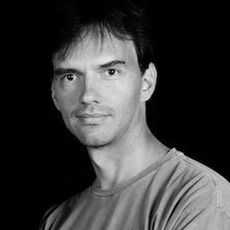
\includegraphics[width=2.6cm,height=2.6cm]{Images/Introduction/ErnestoBaschny.jpg}
			\end{figure}
		\end{column}

	\end{columns}

\end{frame}

% ------------------------------------------------------------------------------
% TYPO3 CMS 6.2 LTS: The Facts (2)
% ------------------------------------------------------------------------------

\begin{frame}[fragile]
	\frametitle{Introductie}
	\framesubtitle{TYPO3 CMS 6.2 LTS: De feiten}

	\begin{itemize}
		\item Release datum: 25 maart 2014
		\item Ontwikkel en release timeline:
	\end{itemize}

	\begin{figure}
		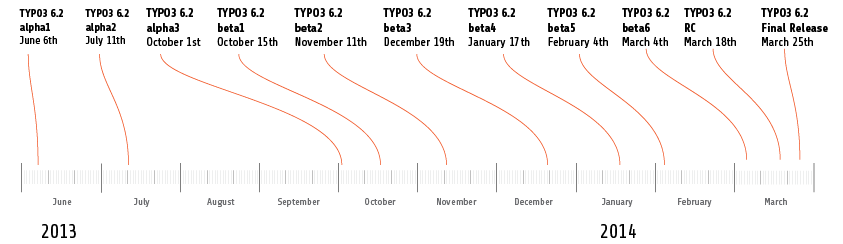
\includegraphics[width=0.99\linewidth]{Images/Introduction/ReleaseTimeline.png}
	\end{figure}

\end{frame}

% ------------------------------------------------------------------------------
% TYPO3 CMS 6.2 LTS: The Facts (3)
% ------------------------------------------------------------------------------

\begin{frame}[fragile]
	\frametitle{Introductie}
	\framesubtitle{TYPO3 CMS 6.2 LTS: The Facts}

	\begin{itemize}
		\item Systeemvereisten 
		\begin{itemize}
			\item PHP	\tabto{1.2cm} v5.3.7 - v5.5.x
			\item MySQL	\tabto{1.2cm} v5.1.x - v5.6.x
		\end{itemize}
	\end{itemize}

	\begin{itemize}
		\item Eind van het onderhoud: maart 2017
		\item TYPO3 CMS 6.2 is een \textbf{Long Term Support} (LTS) release (3 jaar lang ondersteuning!)
	\end{itemize}

\end{frame}

% ------------------------------------------------------------------------------
% TYPO3 CMS 6.2 LTS: The Facts (4) - Release Agenda
% ------------------------------------------------------------------------------

\begin{frame}[fragile]
	\frametitle{Introductie}
	\framesubtitle{TYPO3 CMS 6.2 LTS: De feiten}

	\begin{itemize}
		\item TYPO3 CMS release agenda:
	\end{itemize}

	\begin{figure}
		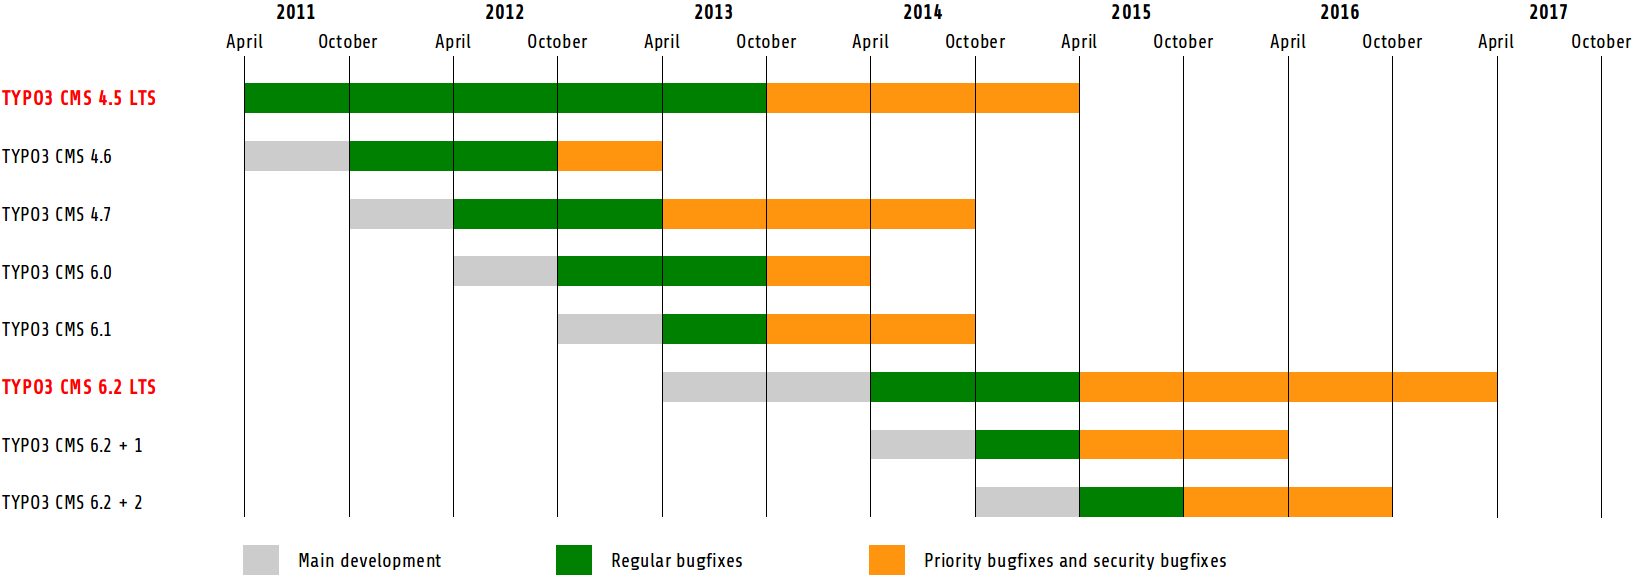
\includegraphics[width=0.99\linewidth]{Images/Introduction/ReleaseAgenda.png}
	\end{figure}

\end{frame}

% ------------------------------------------------------------------------------

